\documentclass[a4paper]{scrreprt}
\usepackage[german]{babel}
\usepackage[utf8]{inputenc}
\usepackage{graphicx}
\usepackage{pdflscape}

\begin{document}
\title{Implementierungsdokument}
\author{Hanselmann, Hecht, Klein, Schnell, Stapelbroek, Wohnig}
\date{\today\\v0.2}
\maketitle 
\tableofcontents	
\listoffigures


\chapter{Einleitung}
Dieses Dokument beschreibt die Implementierungsphase einer Praxis der Softwareentwicklungsgruppe am Karlsruher Institut für Technologie. Der Titel der Gruppenaufgabe lautet: \textit{Entwicklung eines Werkzeugs zur Analyse formaler Eigenschaften von Wahlverfahren}. \\
Diese Dokument stellt die in dieser Phase entstandenen Unterschiede zu den vorherigen Phasen (Pflichtenheft und Entwurf) dar und erklärt, warum diese notwendig wurden. \\
Weiterhin wird die zeitliche sowie die personelle Aufteilung der Implementierung vorgestellt. \\
\section{Ziel des Programmes}
Ziel des Programmes ist es eine Lösung zur Analyse von formalen Eigenschaften von Wahlverfahren zu präsentieren. Zur Analyse der Eigenschaften wird Bounded Model Checking (Glossareintrag) verwendet. Der verwendete Bounded Model Checker ist CBMC (Glossareintrag). Das Programm soll folgende Module  bereitstellen: 
\begin{itemize}
\item Eine Möglichkeit zur Beschreibung eines Wahlverfahrens in der Programmiersprache C. 
\item Eine Möglichkeit zur Beschreibung von Eigenschaften, auf die das Wahlverfahren geprüft werden soll. Die Beschreibung erfolgt in einer Makrosprache (Glossareintrag).
\item Eine Möglichkeit zum Angeben der Parameter für welche das angegebenen Wahlverfahren analysiert werden soll (Anzahl Wähler, Anzahl Kandidaten, Anzahl Sitze). 
\item Eine Möglichkeit, die Analyse auszuführen.
\item Eine Ausgabe des Ergebnisses der Analyse: Eine Erfolgsmeldung falls alle Eigenschaften erfüllt werden und Präsentation eines Gegenbeispiels sonst.
\end{itemize}


\chapter{Unterschiede zu den im Pflichtenheft gestellten Kriterien}

\section{Kannkriterien}

\subsection{/FK1140/- Durch den User konfigurierbares Verhalten C-Editor}
Die Interfaces um diese Anforderungen zu implementieren existieren zwar, es fehlt allerdings an der Zeit dies jetzt noch fertig zu stellen (6-8 Mannstunden).

\subsection{Betrieb auf dem Betriebssytem MacOS} 
Da wir keinen MAC zum testen hatten haben wir keine Implementation für MacOS
vorgenommen. Da unser Entwurf Erweiterungen aber leicht zulässt, ist es für
Benutzer die dieses Betriebssytem besitzen mit einigen Programmierkenntnisse
möglich sich diese Option selbst einzubauen.

\chapter{Änderungen am Entwurf}
\section{highlevel}

AbstractFactory in highlevel ist jetzt keine Abstrakte Fabrik mehr.\\ Dieses Entwurfsmuster konnte nicht verwendet werden, da die zu erstellenden Objekte teilweise voneinander abhängig sind. Weiterhin gibt es Objekte, die mehrere Rollen einnehmen, d.h. sie implementieren unterschiedliche Interfaces (wie etwa der Parametereditor, der sowohl ParameterSource, als auch ProjectSource und MainNotifier implementiert). \\
Deshalb wurde sie durch das Interface CentralObjectProvider und PSECentralObjectProvider, der dieses implementiert, ersetzt. CentralObjectProvider verwirklicht die ursprüngliche Funktion der Abstrakten Fabrik, unabhängig von konkreten Implementierungen zu sein. \\
PSECentralObjectProvider erzeugt die konkreten Objekte für unsere Implementierung der highlevel Interfaces und stellt diese dem BEASTCommunicator zur Verfügung. Dieser muss weiterhin nur von den Interfaces wissen. \\
\\
Es wurde das Interface DisplaysStringsToUser hinzugefügt. Es wird von allen Elementen, die dem Nutzer Text anzeigen, implementiert. Damit wird die Einbindung anderer Sprachen vereinfacht. \\
\\
Allen Interfaces zu Paketen mit GUI wurden die Methoden stopReacting() und resumeReacting() hinzugefügt. Diese verhindern, dass der Nutzer während einer laufenden Analyse Änderungen an dafür benötigten Daten vornimmt. \\
\\
Es wurde das Interface ProjectSource hinzugefügt. Es wird von ParameterEditor implementiert. Damit wird es möglich das Speichern und Laden von ganzen Projekten in zukünftigen Versionen leichter einem anderen Fenster als dem Parametereditor zu überlassen. \\
\\
Interfaces zu Paketen, die Daten für die Analyse bereitstellen, wurde die Methode isCorrect() hinzugefügt. Damit kann vor Start einer Analyse überprüft werden, ob die bereitgestellten Daten frei von Fehlern sind, die die Analyse beeinträchtigen würden.


\section{CodeGenerierung}

Die Klasse CBMCCodeGeneration ist nicht mehr statisch. \\
Sie wird in der Implementierung von der Klasse CBMCProcessFactory instantiiert. \\
So wird für jedes erzeugte C-Tempfile (Glossareintrag) eine neue Instanz erstellt. Sinnvoll, da es es genau von den Parametern abhängt. \\
Jede Instanz der Klasse CBMCCodeGeneration erstellt eine Instanz eines CBMCCodeGenerationVisitor. \\
Dieser besitzt 2 neue Methode, die einstellen ob er zur Codegenerierung einer Vor- oder Nachbedingungen eines Wahlverfahrens verwendet wird.  \\
(Verändertes Klassendiagramm hier)

\section{UserActions}
Alle \verb!UserActions! der vier GUIs haben jetzt nur noch einen Verweis auf den ihnen zugehörigen Controller, und holen sich von diesem mit Gettern die von ihnen gebrauchten Klassen (FileChooser, SaveBeforeChangeHandler..). Beispielhaft am \verb!BooleanExpEditor! gezeigt:
\newline

(Diagramm folgt)
\newline

\section{SaverLoader}
PostAndPrePropertiesDescriptionSaverLoader, ElectionDescriptionSaverLoader, ParameterCheckParameterSaverLoader und ProjectSaverLoader implementieren nun das Interface SaverLoader mit den dargestellten Methoden. Dies ermöglicht es der Klasse FileChooser, polymorph gegebene DatenTypen abzuspeichern und gegebene Dateien zu laden.
Alle anderen \verb!SaverLoader!-Klassen haben nur statische Methoden.
Zudem gibt es noch eine \verb!StringSaverLoader! Klasse die mit \verb!createSaveString! aus allen vom Nutzer editierbaren Strings alle Vorkommen von ">" durch ">>" ersetzt, bzw. dies mit !\verb!createFromSaveString! rückgängig macht. Dies verhindert die Erstellung von nicht ladbaren Dateien trotz validen Nutzer-Eingaben.
\newline
(Diagramm folgt)
\newline

\section{FileChooser}
Diese Klasse kümmert sich um das Laden und Speichern der speicherbaren Datentypen.
\newline
(Diagramm folgt)
\newline

\section{DataTypes}
Die als Datei abspeicherbaren Datentypen implementieren nun alle das Interface \verb!ChangeNameInterface!, dass es dem \verb!FileChooser! ermöglicht das name-Attribut dieser Klassen polymorph zu verändern.
\newline
(Diagramm folgt)
\newline


\section{Codearea}
- Errordisplayer ist nun abstrakt. Von den erbenden Klassen müssen Fehlermeldungen generiert werden.\\
- Klasse SaveTextBeforeRemove wurde hinzugefügt. Diese speichert den Text einer JTextPane sobald Text daraus entfernt wird. Dies ist nötigt da das RemovedUpdate des Styleddocuments keinen Zugriff auf den entfernten Text gewährt. Dieser ist jedoch benötigt um Aktionen rückgängig zu machen. Implementiert wird die Funktionalität durch hören auf Keyevents.\\
- Klasse TextLineNumber hinzugefügt, welche die Zeilennummer anzeigt. Diese Klasse wurde direkt aus https://tips4java.wordpress.com/2009/05/23/text-component-line-number/ übernommen\\
- Klasse SquigglePainter wurde hinzugefügt. Diese unterstreicht Text in der JTextPane gezackt. Dies wird verwenden um Fehler im Code anzuzeigen. Übernommen von 
https://tips4java.wordpress.com/2008/10/28/rectangle-painter/\\
- Klasse JTextPaneToolbox wurde hinzugefügt. Diese enthält einige statische Methoden welche oft benötigte, aber nicht zusammengehörige Funktionalität für JTextPane liefern. Dazu gehört u.a. das umwandeln absoluter Positionen in Zeilennummern.\\
- Tabinserter wurde hinzugefügt. Dieser fügt Tabs in Form von Leerzeichen ein.\\
- Inteface LineBeginningTabsHandler und Implementierung CurlyBracesLineBeginningTabHandler wurden hinzugefügt. LineBeginningTabsHandler berechnet die benötigte Anzahl Tabs zu Beginn einer gegebenen Zeile. CurlyBracesLineBeginningTabHandler errechnet dies anhand der Anzahl '{' in vorangehenden Zeilen minus die Anzahl } am ende der gegebenen Zeile\\
- Es gibt nun spezielle Useractions für Kopieren, Ausschneiden und Einfügen. Dies ist nötig um sicher zu stellen dass nicht editierbare Zeilen nicht verändert werden durch diese Aktionen.

\subsection{UserInsertToCode}
Hinzu kommen folgende Funktionen:
\begin{itemize}
\item insertTab fügt an der Momentanen Position ein Tab ein
\item insertChar Fügt das gegebene Zeichen an der momentanen Position ein
\item getFirstLockedLine gibt die erste nicht editierbare Zeilennummer
\item moveToEndOfCurrentLine Bewegt den Caret ans Ende der momentanen Zeile
\item moveToStartOfCurrentLine Bewegt den Caret an den Start der momentanen Zeile
\item removeToTheRight Entfernt das Zeichen rechts vom Caret
\item removeToTheLeft Entfernt das Zeichen links vom Caret
\end{itemize}
Entfernt wurden:

\begin{itemize}
\item msgLockedLinesListeners: wird nun von LockedLineHandler übernommen
\end{itemize}

\section{BooleanExpEditor}
Besitzt jetzt eine Referenz auf die \verb!CElectonDescriptionEditor!-Instanz, da dies zur Fehlerfindung durch den \verb!BooleanExpEditorVariableErrorFinder! nötig ist
\newline
(Diagramm folgt)
\newline

\section{CElectionDescriptionEditor}

Die \verb!ChangeElectionType! \verb!UserAction! und der entsprechende Menüpunkt "Wahlart ändern" wurden entfernt, da es sehr wenig Sinn macht ein bestehendes Wahlverfahren grundsätzlich zu ändern anstatt einfach ein neues zu erstellen und die Implementierung dieser \verb!UserAction! somit unnötig kompliziert wäre.
\newline
(Diagramm folgt)
\newline
Neues Package ElectionTemplates kam hinzu. Dises enthält folgende Klassen\\
ElectionTemplateHandler: Gibt alle Election Input und Output datentypen und deren ids aus\\
ElectionTemplateChooser: Zeigt dem Benutzer einen Dialog welcher es ermöglicht Input und result eines neuen Wahlverfahrens zu wählen

\section{PropertyChecker}

Beim PropertyChecker haben sich folgende Sachen im Vergleich zum Entwurf
verändert:
\begin{itemize}
\item Die Klasse CBMC\_Result besitzt nun die Methode ``createFailureExample''
  samt zugehöriger Untermethoden, welche zur Erstellung des Failurexamples
  genutzt werden. Deshalb besitzt die Klasse Checker diese Fähigkeit nicht mehr.

\item Es wurden drei neue Klassen namens
``CBMC\_Result\_Wrapper\_/long/singleArray/multiArray'' erstellt. Diese werden
während des parsens der Rückgabe von CBMC verwendet um die Teilergebnisse in
Listen zu speichern und sie dann am Ende als Array ausgeben zu können. Dies
wurde auf diese Weise implementiert, da am Anfang des parsens nicht bekannt
sein kann, wie groß die Datentypen bei der Rückgabe werden würden und es die
eigentliche Methode ``createFailureExample'' deutlich verkürzen konnte.

\item Die Klasse CheckerFactory besitzt nun die zwei neue Methoden: \newline
``getNewInstance(\ldots)'' wird dazu verwendet eine neue Instanz einer
Checkerfactory zu erstellen, damit die CheckerFactoryFactory neue CheckerFactory
erstellen kann. \newline Außerdem gibt es nun die Methode ``getMatchingResult(int
amount)'' welche die gewünschte Anzahl an Checkerspezifischen Result Objekten
zurückgibt, sodass die CheckerFactoryFactory von diesen dann auf Wunsch so viele
wie nötig erstellen kann.

\end{itemize}


\section{PropertyList}

Das Package PropertyList hat sich hauptsächlich im Subpackage Controller geändert. Durch die Anbindung an die High-Level-Interfaces wurde es nötig, dass das Model der PropertyList kein Singleton mehr ist. Der Controller benötigt deshalb eine eigene Referenz auf das Model. Eine zentrale Controllerklasse übernimmt nun die Steuerung, anstatt wie vorgesehen einzelne Klassen.

Die Methoden für Controller und Model wurden außerdem in eigenen Interfaces beschrieben, sodass ein schneller Überblick möglich ist.

\subsection{Model}
Die Klasse PropertyList wurde zum "`PLModel"' umbenannt. Sie hat keine Anbindung nach außerhalb des Packages mehr. Das Interface PostAndPrePropertiesDescriptionSource wird nun vom Controller implementiert.

Die Klasse "`PropertyItem"' hält nun zusätzlich Daten zum Ergebnis der Analyse (zusätzlich zu PropertiesDescription und Teststatus).

Das Interface "`PLModelInterface"' beschreibt alle Manipulationen für die Eigenschaftenliste.

\subsection{Controller}
Die zentrale Klasse des Controllers heißt "`PropertyList"' und implementiert alle nötigen Interfaces nach außen. Das sind:
\begin{itemize}
	\item ResultPresenter (im Entwurf nur vom View implementiert)
	\item PostAndPrePropertiesDescriptionSource (eigentlich im Entwurf im Model implementiert)
	\item Runnable (Klasse startet den View)
	\item DisplaysStringsToUser (zur Entgegennahme der Strings für den View)
	\item PLControllerInterface (alle möglichen Befehle für die PropertyList)
\end{itemize}
Die Action- und Changelistener wurden aus dem Controller rausgezogen und direkt im View implementiert.

Die Klassen, die "`ListChangeCommand"' erweiterten (ChangeDescription, ChangeDescriptionName, AddStandardDescription, AddNewDescription, ChangeTestedStatus, Redo, Undo), sind nur noch Methoden im Interface des Controllers (void changeName(PropertyItem prop, String newName); usw.). Das geschah, weil sie so kleine Änderungen an der PropertyList bedeuten, dass sie nicht rückgängig gemacht werden müssen. Stattdessen kann der Nutzer neu erstellte Eigenschaften mit dem Klick auf den entsprechenden Button wieder löschen. Lediglich "`DeleteDescriptionAction"' ist den Undo wert und wurde deshalb in einer eigenen Klasse gekapselt.

Der "`SaveBeforeChangeHandler"' war im Entwurf noch nicht beschrieben.

\subsection{View}
Die Elemente des View sind zum großen Teil gleich geblieben. Sie wurden allerdings nicht mit einem GUI-Builder erstellt, weil dann nicht dynamisch Komponenten hinzugefügt werden hätten können (Formulare mit fester Anzahl von Komponenten).

Im Entwurf war angedacht, dass das Model die View direkt von Änderungen benachrichtigt. Nun wird das Observer-Pattern benutzt, um dem View Änderungen im Model mitzuteilen. In diesem Falle wird die Liste der Eigenschaften (ArrayList<ListItem>) neu aufgebaut.

Die Komponenten können aufhören, auf Benutzereingaben zu reagieren und wieder anfangen.

Der Container der "`ListItem"' wurde zu einem JPanel.

Neu hinzugekommen ist die Klasse "`ResultPresenterWindow"' , die die Swing-Klasse "`JFrame"' erweitert. Dadurch war es nicht möglich, sie als Kinder des Hauptfensters zu deklarieren. Aber durch die Entscheidung gegen eine "`JTextPane"' konnte das Layout aus dem Pflichtenheft besser dargestellt werden.

\section{Parametereditor}

Die Klasse ParameterEditor implementiert jetzt nicht mehr BEASTCommunicator aus highlevel. Damit wird ParameterEditor klar von der Kommunikation zwischen den einzelnen Teilen von BEAST getrennt. \\
\\
Es wurden neue UserActions hinzugefügt:
\begin{itemize}
\item NewProjectUserAction, um neben Laden und Speichern auch das Erstellen eines neuen Projekts zu ermöglichen.
\item OptionsUserAction, um es dem Nutzer zu ermöglichen, Einstellungen wie etwa die Sprache zu ändern.
\item ShowHideBooleanExpEditor, ShowHideCElectionEditor und ShowHidePropertyList um die anderen GUI-Fenster vom Parametereditor aus öffnen und schließen zu können.
\end{itemize}
Es wurden neue Handler hinzugefügt:
\begin{itemize}
\item ArgumentHandler, um die benutzerdefinierten Argumente für CBMC zu verarbeiten.
\item SaveBeforeChangeHandler, um sicherzustellen, dass der Nutzer nicht versehentlich durch Laden oder Erzeugen eines neuen Projekts ein ungespeichertes Projekt verwirft
\end{itemize}


\chapter{Zeitablauf Implementierungsphase}

\section{Geplanter Ablauf}

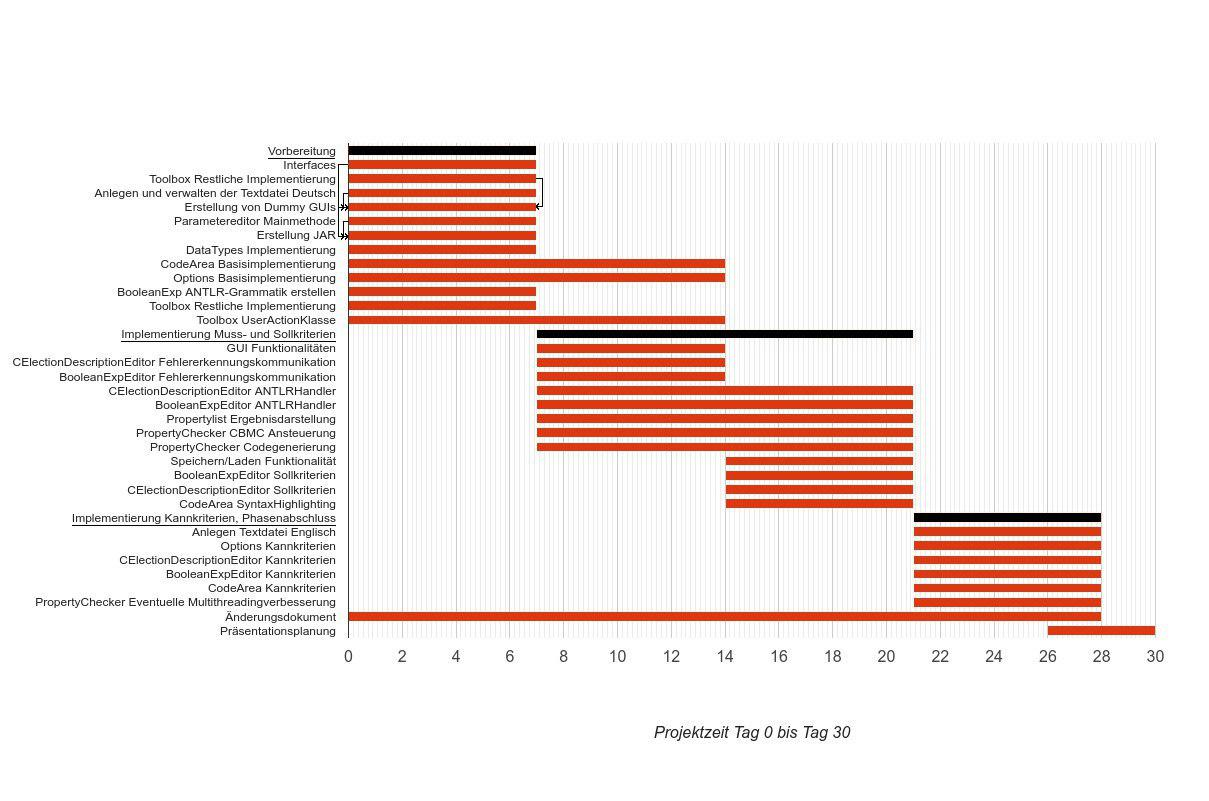
\includegraphics[width=1.3\textwidth] {originalPlanung.jpg}

\section{Eigentlicher Ablauf}
Der ursprüngliche Plan wurde hauptsächlich eingehalten. Ein Paar Komplikationen bei den Paketen \verb!highlevel!, \verb!parametereditor! und \verb!propertylist! verzögerten die Fertigstellung einiger Meilensteine.

(Genauere Beschreibung von Aufgabenumverteilung bzw. Ablaufänderung folgt)

(GANTT Diagramm von tatsächlichem Ablauf folgt)

\end{document}